%==============================================================================
% TEMPLATE FOR THESIS WAGENINGEN UNIVERSITY
% CREATED BY AREND LIGTENBERG JUNE 2006;
% EDITED BY KIM CALDERS 2014;
% EDITED BY BEN DEVRIES 2015;
% EDITED BY LOIC DUTRIEUX 2016
%==============================================================================

\documentclass [a4paper,12pt,twoside]{book}
%Putting my additions here, friend
\usepackage{epstopdf}
\usepackage{threeparttable}
\usepackage[running]{lineno}
\usepackage{threeparttablex}

\usepackage[utf8]{inputenc}
\usepackage[dutch,english]{babel}
\usepackage{graphicx}
\usepackage{natbib}
\usepackage{bibentry}
\nobibliography*
\usepackage{amsmath}
\usepackage{fancyhdr}
\usepackage[small,bf]{caption}
%\captionsetup[table]{skip=10pt}
\usepackage{multirow}
%\usepackage[body={6.0in, 8.2in},left=1.50in,right=1.50in]{geometry} %% very narrow
\usepackage[top=3.35cm, bottom=3.35cm, left=2.5cm, right=2.5cm]{geometry}
\usepackage[parfill]{parskip}
\usepackage{enumitem}
%\usepackage[rightcaption]{sidecap}
%\usepackage{epstopdf}
\usepackage{pdfpages}
%\usepackage[hidelinks]{hyperref}
\usepackage{color}
\usepackage{appendix}

% extra packages added by Ben
\usepackage{rotating} % for rotating figures
\usepackage{changepage} % for indenting entire paragraphs
\usepackage{float} % help with table positioning
\floatstyle{plaintop} % caption on top
\restylefloat{table} % see above. Use: \begin{table}[H]
\usepackage{textcomp} % \textdegree
\usepackage{fixltx2e} % for the \textsubscript command outside of a math environment
\usepackage{csquotes} % for block quotes, use {displayquote} environment
\usepackage{todonotes}
\usepackage{soul}
\usepackage{fp}
\usepackage{tabularx}
\usepackage{subcaption}
\usepackage{pdflscape}
\usepackage{gensymb}
\usepackage{mhchem}
\usepackage{wrapfig}


\addto\captionsenglish{\renewcommand{\bibname}{References}}

\definecolor{Red}{rgb}{0.5,0,0}
\definecolor{Blue}{rgb}{0,0,0.5}


%=======================================================================
% GENERAL SETTINGS
%=======================================================================
%\oddsidemargin 40pt
%\evensidemargin 40pt
\setlength{\captionmargin}{5pt}
%\setlength{\textfloatsep}{10pt plus 1.0pt minus 2.0pt}
%\usepackage{pifont}
%\usepackage{times}
%\usepackage{txfonts}
%\usepackage[sc]{mathpazo}
%\usepackage{setspace}

\linespread{1.1} %1 is single spacing, 1.3 is oneandhalf spacing


%\citationstyle{dcu}
\sloppy
\setcounter{tocdepth}{0}

%% for internal use
\newcommand{\fixme}[1]{\emph{\marginpar{FIXME} (#1)}}
\newcommand{\readme}[1]{\emph{\marginpar{README} (#1)}}
\newcommand{\verifyme}[1]{\emph{\marginpar{VERIFYME} (#1)}}


%=======================================================================
% DEFINITION OF THE FANCY HEADERS
%=======================================================================
\pagestyle{fancy}
\renewcommand{\chaptermark}[1]{\markboth{#1}{}}
\renewcommand{\sectionmark}[1]{\markright{\thesection\ #1}}
\fancyhf{}
\fancyhead[LE,RO]{\bfseries\thepage}
\fancyhead[LO]{\bfseries\rightmark}
\fancyhead[RE]{\bfseries\leftmark}
%\fancyfoot[LE,CE,RE]{\scriptsize{Draft: June 2006}}
%\fancyfoot[LO,CO,RO]{\scriptsize{Draft: June 2006}}
\headheight 15pt

\fancypagestyle{plain}{%
\fancyhead{} % get rid of headers
\renewcommand{\headrulewidth}{0pt} % and the line
}
\renewcommand{\headrulewidth}{0.4pt}
%\renewcommand{\footrulewidth}{0.4pt}

\pdfinfo{
   /Author (John Doe)
   /Title  (Title of your thesis)
   /CreationDate (D:Date)
}

%=======================================================================
% NEW ENVIRONMENT FOR THE START OF CHAPTER (SMALL ABSTRACT)
%=======================================================================
\newenvironment{chapintro}
{
    \begin{center}
    \begin{minipage}[t]{0.9\textwidth}
    \hrule
    \medskip
    \small
}
{
    \medskip
    \hrule
    \end{minipage}
    \end{center}
    \bigskip
}


%=======================================================================
% ADD WORD CHAPTER FOR TOC
%=======================================================================


\makeatletter
\let\orig@chapter\@chapter
\def\@chapter[#1]#2{\ifnum \c@secnumdepth >\m@ne
                       \if@mainmatter
                         \refstepcounter{chapter}%
                         \typeout{\@chapapp\space\thechapter.}%
                         \addcontentsline{toc}{chapter}%
                                   {Chapter~\protect\numberline{\thechapter}#1}%
                       \else
                         \addcontentsline{toc}{chapter}{#1}%
                       \fi
                    \else
                      \addcontentsline{toc}{chapter}{#1}%
                    \fi
                    \chaptermark{#1}%
                    \addtocontents{lof}{\protect\addvspace{10\p@}}%
                    \addtocontents{lot}{\protect\addvspace{10\p@}}%
                    \if@twocolumn
                      \@topnewpage[\@makechapterhead{#2}]%
                    \else
                      \@makechapterhead{#2}%
                      \@afterheading
                    \fi}
\makeatother

%=======================================================================
% A BIT MORE COMPACT ITEM LIST
%=======================================================================
\newenvironment{itemize*}%
  {\begin{itemize}%
    \setlength{\parskip}{0pt}%
    \setlength{\itemsep}{0pt}%
    \setlength{\parsep}{0pt}}%
  {\end{itemize}}

%more compact enumeration list
  \newenvironment{enumerate*}%
  {\begin{enumerate}%
    \setlength{\itemsep}{0pt}%
    \setlength{\parskip}{0pt}}%
  {\end{enumerate}}

%=======================================================================
% A BIT MORE COMPACT DESCRIPTION LIST
%=======================================================================
\renewcommand{\descriptionlabel}[1]{\hspace{\labelsep}\textrm{#1}}

\newenvironment{description*}%
  {\begin{description}%
    \setlength{\itemsep}{0pt}%
    \setlength{\parskip}{0pt}}%
  {\end{description}}

%=======================================================================
% A BIT MORE COMPACT BIBLIOGRAPHY
%=======================================================================
  \let\oldthebibliography=\thebibliography
  \let\endoldthebibliography=\endthebibliography
  \renewenvironment{thebibliography}[1]{%
    \begin{oldthebibliography}{#1}%
      \setlength{\parskip}{0ex}%
      \setlength{\itemsep}{1ex}%
  }%
  {%
    \end{oldthebibliography}%
  }

%=======================================================================
% CLEAR HEADER STYLE ON LAST EMPTY ODD PAGES
%=======================================================================
\makeatletter
\def\cleardoublepage{\clearpage\if@twoside \ifodd\c@page\else%
\hbox{}%
\thispagestyle{empty}%
\newpage%
\if@twocolumn\hbox{}\newpage\fi\fi\fi}
\makeatother


%=======================================================================
% SOME EXTRA COMMANDS FOR VISUAL LAYOUT
%=======================================================================
\newcommand{\longpage}{\enlargethispage{\baselineskip}}
\newcommand{\shortpage}{\enlargethispage{-\baselineskip}}
\newcommand{\setreference}{\vspace*{\fill}}

%=======================================================================
% LIST ENVIRONMENT FOR OWN SELECTED PUBLICATIONS
%=======================================================================
\newenvironment{pubs}
{
\begin{list}{}
{%
\item[]}%
\setlength{\itemindent}{-25pt}%
\setlength{\parsep}{-0pt}
\setlength{\itemsep}{-0pt}
}%
{\end{list}%
}%


%==============================
% REFORMAT SECTION HEADINGS
%==============================

%% using titlesec
\usepackage{titlesec}
%% FIX FOR BUG in titlesec 2.10.1
\usepackage{etoolbox}

\makeatletter
\patchcmd{\ttlh@hang}{\parindent\z@}{\parindent\z@\leavevmode}{}{}
\patchcmd{\ttlh@hang}{\noindent}{}{}{}
\makeatother
%% END OF BUGFIX

\titleformat{\subsection}
  {\normalfont\normalsize\bfseries}
  {\thesubsection}{1em}{}
\titleformat{\subsubsection}
  {\normalfont\normalsize\itshape}
  {\thesubsubsection}{1em}{}



%==============================
% Force start of newpage on left page
%==============================
\newcommand*\cleartoleftpage{%
  \clearpage
  \ifodd\value{page}\hbox{}\newpage\fi
}



%=======================================================================
% INCLUSION OF THE CONTENT
%=======================================================================

\raggedbottom % preferentially leaves whitespace at bottom of page instead of distributing throughout vertical space

\begin{document}

\frontmatter
\pagenumbering{alph}
\pagenumbering{roman}
\addtocontents{toc}{~\hfill\rlap{\textbf{Page}}\par}
\thispagestyle{empty}
%%%%%%%%%%%%%%%%%%%%%%%%%%%%%%%%%%%%%%%%%%%%%%%%%%%%%%%%%%%%%%%%%%
\begin{center}
\Huge{\textbf{A Statistical Evaluation of}} \\
\Huge{\textbf{Hybrid Potato Breeding}} \\
\vspace*{1cm}
\vspace*{1cm}
\vspace*{\fill}
\large{James R. Adams}\\
\end{center}

%%%%%%%%%%%%%%%%%%%%%%%%%%%%%%%%%%%%%%%%%%%%%%%%%%%%%%%%%%%%%%%%
\newpage
\thispagestyle{empty}
\vspace*{\fill}
\begin{tabular}{l}
    \textbf{Thesis committee}                                                                 \\  
                                                                                              \\  
    \textbf{Promotor:}                                                                        \\  
    Prof.dr J. Smith                                                                          \\  
    Professor of Geo-information Science and Remote Sensing                                   \\  
    Wageningen University                                                                     \\  
                                                                                              \\  
    \textbf{Co-promotors:}                                                                    \\  
    Dr. Name of co-promotor                                                                   \\  
    Assistant Professor, Laboratory of Geo-information Science and Remote Sensing             \\  
    Wageningen University                                                                     \\  
                                                                                              \\  

    \textbf{Other members:}                                                                   \\  
    Prof.dr Jury member 1, Wageningen University                                              \\  
    Prof.dr Jury member 2, Affiliation                                                        \\  
    Prof.dr Jury member 3, Affiliation                                                        \\  
    Prof.dr Jury member 4, Affiliation                                                        \\  
                                                                                              \\  

    \small{This research was conducted under the auspices of the C.T. de Wit Graduate School} \\  
    \small{of Production Ecology \& Resource Conservation (PE$\&$RC)}                         \\  
\end{tabular}

%%%%%%%%%%%%%%%%%%%%%%%%%%%%%%%%%%%%%%%%%%%%%%%%%%%%%%%%%%%%%%%%
\newpage
\thispagestyle{empty}
\begin{center}
\Huge{\textbf{Title of your}} \\
\Huge{\textbf{thesis}} \\
\vspace*{1cm}
\Large{John Doe}\\
\normalsize
\vspace*{\fill}
\textbf{Thesis} \\
submitted in fulfilment of the requirements for the degree of doctor at \\
Wageningen University\\
by the authority of the Rector Magnificus\\
Prof. Dr A.P.J. Mol,\\
in the presence of the\\
Thesis Committee appointed by the Academic Board\\
to be defended in public\\
on Date of your defense\\
at 4 p.m. in the Aula.\\
\end{center}

%%%%%%%%%%%%%%%%%%%%%%%%%%%%%%%%%%%%%%%%%%%%%%%%%%%%%%%%%%%%%%%%%%%
\newpage
\thispagestyle{empty}
\vspace*{\fill}
\begin{flushleft}
\begin{tabular}{l}
    John Doe                                                 \\  
    Title of your thesis                                     \\  
    170 pages.                                               \\  
                                                             \\  
    PhD thesis, Wageningen University, Wageningen, NL (2015) \\  
    With references, with summary in English                 \\  
                                                             \\  
    ISBN XXX-YYY                                             \\  
\end{tabular}
\end{flushleft}
%\newpage
%\thispagestyle{empty}
%\begin{flushright}
%\vspace*{\fill}
%\textit{Aan mijn ouders}
%\end{flushright}

\cleardoublepage
\cleardoublepage
\phantomsection

\addcontentsline{toc}{chapter}{Acknowledgements}
\chapter*{Acknowledgements}

Lorem ipsum dolor sit amet, consectetur adipisicing elit, sed do eiusmod
tempor incididunt ut labore et dolore magna aliqua. Ut enim ad minim veniam,
quis nostrud exercitation ullamco laboris nisi ut aliquip ex ea commodo
consequat. Duis aute irure dolor in reprehenderit in voluptate velit esse
cillum dolore eu fugiat nulla pariatur. Excepteur sint occaecat cupidatat non
proident, sunt in culpa qui officia deserunt mollit anim id est laborum. Lorem ipsum dolor sit amet, consectetur adipisicing elit, sed do eiusmod
tempor incididunt ut labore et dolore magna aliqua. Ut enim ad minim veniam,
quis nostrud exercitation ullamco laboris nisi ut aliquip ex ea commodo
consequat. Duis aute irure dolor in reprehenderit in voluptate velit esse
cillum dolore eu fugiat nulla pariatur. Excepteur sint occaecat cupidatat non
proident, sunt in culpa qui officia deserunt mollit anim id est laborum. Lorem ipsum dolor sit amet, consectetur adipisicing elit, sed do eiusmod
tempor incididunt ut labore et dolore magna aliqua. Ut enim ad minim veniam,
quis nostrud exercitation ullamco laboris nisi ut aliquip ex ea commodo
consequat. Duis aute irure dolor in reprehenderit in voluptate velit esse
cillum dolore eu fugiat nulla pariatur. Excepteur sint occaecat cupidatat non
proident, sunt in culpa qui officia deserunt mollit anim id est laborum.


\newpage
\vspace*{\fill}
\begin{center}
"감자엿이 제일이래

많이 들고 장수하소 장수령감

감자술잔 비우면서 하는 말이"
\\
\\
"The potato taffy is the best they say

  the old man who ate a lot and lived to a ripe old age

      says while emptying a glass of potato liquor . . ."
                                                                                         
                 - Excerpt from "Potato Pride" (감자자랑)
\end{center}
\vspace*{\fill}


\cleardoublepage

\chapter{Summary}
\label{cha:Summary}

Modern potato exists as the culmination of millennium of domestication, selection, and cultivation. Only over the past 100 years have concentrated efforts been made on the genetic improvement of potato.

Potato is prized for its tubers which have become a staple in many cultures, a central ingredient in my industrial applications, and . Potato improvement 

\cleardoublepage
\phantomsection

\addcontentsline{toc}{chapter}{Contents}  
\tableofcontents
\cleardoublepage
\phantomsection
\pagenumbering{arabic} \setcounter{page}{1}


%% Main Chapters
\mainmatter
\setcounter{page}{1}
\include{01_chapter1} % Introduction 
\include{02_chapter2}
\usepackage{bibentry}  % Load the bibentry package
\nobibliography{library}

\chapter[Little heterosis found in Diploid Hybrid Potato | The genetic underpinnings of a new hybrid crop]{Little heterosis found in Diploid Hybrid Potato | The genetic underpinnings of a new hybrid crop}


\chaptermark{Genetic underpinnings of diploid hybrid potato}
\label{cha:chapter2}
\vspace*{\fill}
This chapter is based on:
\\
\\
% Full citation of the published (or submitted/in review) article
% This refers to the article key in the refs.bib file.
\bibentry{Adams2022}
\newpage

\section*{Abstract}
 Hybrid potato breeding has become a novel alternative to conventional potato breeding allowing breeders to overcome intractable barriers (e.g. tetrasomic inheritance, masked deleterious alleles, obligate clonal propagation) with the benefit of seed-based propagule, flexible population design, and the potential of hybrid vigour. Until now, however, no formal inquiry has adequately examined the relevant genetic components for complex traits in hybrid potato populations. In this present study, we use a two-step multivariate modelling approach to estimate the variance components to assess the magnitude of the general and specific combining abilities (GCA and SCA, respectively) in diploid hybrid potato (DHP). SCA effects were identified for all yield components studied here warranting evidence of non-additive genetic effects in hybrid potato yield. However, the estimated GCA effects were on average two times larger than their respective SCA quantile across all yield phenotypes. Tuber number GCA’s and SCA’s were found to be highly correlated with total yield's genetic components. Tuber volume was shown to have the largest proportion of additive and non-additive genetic variation suggesting under-selection of this phenotype in this population. The prominence of additive effects found for all traits presents evidence that the mid-parent value alone is useful for hybrid potato evaluation. Heterotic vigour stands to be useful in bolstering simpler traits but this will be dependent on target phenotypes and market requirements. This study represents the first diallel analysis of its kind in diploid potato using material derived from a commercial hybrid breeding programme.

\section{Key Message}\label{key-message}

Hybrid vigour was detected for multiple traits in diploid hybrid potato. Additive gene action was most prominent in tuber yield and should be the primary target within hybrid breeding programmes.

\newpage

%\runningauthor{JR Adams, ME Vries, C Zheng, \& FA Eeuwijk}
%%% last name of the first author followed by et al, if more than two authors.
%%%\runningauthor{FirstAuthorLastname \textit{et al.}}
%
%\author[$\ast$$\dagger$$\ddagger$]{James R. Adams}
%\author[$\ddagger$]{Michiel E. de Vries}
%\author[$\dagger$]{Chaozhi Zheng}
%\author[$\dagger$]{Fred A. van Eeuwijk}
%
%\affil[$\dagger$]{Biometris, Mathematical and Statistical Methods, Wageningen University and Research, Wageningen, The Netherlands}
%\affil[$\ddagger$]{Solynta, Dreijenlaan 2, 6703 HA, Wageningen, The Netherlands}
%
%\correspondingauthoraffiliation[$\ast$]{Corresponding author: James.adams@wur.nl}
%
%
%\keywords{Diploid hybrid potato; GCA; SCA; Sparse crossing design; heterosis}
%
%\dates{\rec{xx xx, xxxx} \acc{xx xx, xxxx}}
%
%
\linenumbers %to insert line number



\section{Introduction}

Potato (\emph{Solanum tuberosum}), a plant species once isolated to the continents of southern and central America, is now a crop that spans over 17 million hectares of crop-land worldwide \citep{faostat2021}. It is the most prominent of non-cereals and is considered by many a major keystone in guaranteeing food security for both local and global communities. Prized for their edible starch-rich tubers, potato meets the demand of several key industries including the fresh, processing, and seed potato markets with a global gross value of 140.5 billion USD as of 2019. As a field crop, potato has a competitive harvest index of 0.85 (in contrast to 0.4-0.6 seen in other crops) in conjunction with a high water productivity \citep{Hay1995, Lutaladio2009}. There is also ample variation in potato's tuberization timing requiring as few as 75 days from planting to harvest. All the above make potato a highly productive crop amenable to a variety of cropping systems capable of supplying valuable starch with less agronomic input.

Despite potato's growing economic and societal importance, rates of crop improvement in complex traits have not kept in step with other major crops over the past century \citep{Douches1996, Hirsch2013}. Reasons for these deficits in genetic gain are numerous (e.g.~market segmentation, large inventory of quality traits, etc.) but many of them stem from the complexities of potato's evolution and domestication. Potato's tetraploidy is an oft-cited stumbling block for breeders impeding the ability to fix beneficial loci, and conversely, remove deleterious sites harboured across the genome \citep{Lian2019, Zhang2019}. Not only does polyploidy mask deleterious loci from traditional forces of selection, but it also impacts the length of time for site fixation even under genetic drift leading to greater maintenance of heterozygosity over time \citep{Bartlett1934}. Taken together with a very strong self-incompatibly mechanism, potato could best be described as a fortified heterozygous out-crosser. These biological realities shaped potato breeding from the beginning with breeders conducting crosses between promising heterozygous individuals followed by the evaluation of large nurseries in search for decent complementation \citep{Simmonds1979}. These F1 nurseries were then subjected to as many as eight subsequent rounds of clonal selection until only elite candidates were left \citep{Bradshaw2017}. While in some ways this method of clonal breeding is quite efficient (all genetic factors are effectively \emph{fixed} at the creation of the F1), it is widely known for being a long process from generation of the nursery to variety release. Because the success of clonal breeding is highly dependent on the generation of enough novel genotypes in the F1, it takes as many as 9 years to sufficiently bulk tubers in conjunction with applying appropriate selection pressure \citep{Bryan1981, Tai1984}. It should be noted that while there have been proposals to optimise conventional clonal breeding \citep{Neele1991, Bradshaw2003}, many of the aforementioned issues are simply implicit to breeding tetraploid potato.

One solution to this comprehensive set of challenges is the adaptation of potato from a tetraploid clonal crop to that of a diploid inbred-hybrid one, an idea which has existed in some form for over 60 years \citep{Hougas1958}. The benefits of such a change, if possible, are manifold; Diploids only take one generation to half their heterozygosity in contrast to an autotetraploid which takes upwards of four generations making the production of pure-breeding lines plausible in the former. As an extension of this, superior genetic performance in the final marketed variety is not dependent on a single crossing event that generated the original F1 (as it is in conventional clonal breeding) but is accomplished through multiple stages (e.g.~parental pool improvement, parental line development, hybrid crossing, etc.). This is not to mention other logistical niceties such as the ease of producing \& storing true potato seed over vegetative propagule \citep{Cock1983, Pallais1991, Thomas-Sharma2016}. Despite the potential of diploid potato, however, it was not until the cusp of the 21st century that it became broadly feasible. Many picked up on the work of \citep{Hosaka1998} and began the process of generating self compatible populations through the use of \emph{Sli}. \citep{Lindhout2011} was one of the first to confirm the commercial viability generating diploid potato populations capable of inbreeding using a \emph{Sli} donor. Several subsequent studies not only corroborated that inbred populations in diploid potato were possible \citep{Alsahlany2021}, but hybrids generated from these populations resulted in a crop that could compete in the same space as tetraploid potato \citep{Stockem2020, Zhang2021}. While diploid hybrid potato (DHP) populations are now extant across the world, there is at this time little known about the genetic components controlling complex traits as DHP is still a young hybrid crop. Understanding this is an imperative for potato breeders in order to structure breeding programmes which are able to best exploit the genetic variation available to DHP.

We set out to inspect tuber yield in a large DHP test-cross. To do this, we performed a joint evaluation of total yield along with two of its simpler yield components, average tuber volume and total tuber number, and partitioned their underlying genetic effects into additive and non-additive components. This trait and genetic decomposition was done to inspect two broad questions: (1) Which tuber phenotypes in this population were responsible for the variation seen in total yield and (2) are these yield phenotypes primarily under the control of additive or non-additive gene action? This latter question holds particular weight as it gives insight on where the focal point of DHP breeding should lie. We put forward a two-part modelling approach to utilise intra-block information to estimate the general and specific combining abilities of our hybrid parents and crosses, respectively. Our study presents the first diallel study in DHP using highly-inbred parents derived from a commercial breeding programme.


\section{Materials and methods}
\label{sec:materials:methods}

\subsection{Crosses and Trials}

A panel of 400 inbred parents were selected and crossed according to distinct selection criteria related to fertility and agronomic traits yielding 806 successful F1 crosses. These parents were produced from an experimental population derived from several backgrounds including \emph{tuberosum} and several wild species (e.g.~\emph{Solanum chacoense}) \citep{Lindhout2018}. In the Spring of 2019, all hybrid TPS were sown in trays and grown out in a greenhouse. In May, all seedlings were transplanted at stage 105 development (See \citep{Kacheyo2021}) into two field trials located in the Dutch towns of Est and Heelsum. Both trials utilised a double ridge design with eight plants per ridge with a total of sixteen plants per plot; this design was chosen to minimize within-plot variation while reducing planting costs across each trial \citep{Stockem2021}. Plots were organised in an augmented randomised complete block design with two blocks and three internal controls used across each block. All 806 F1 hybrids were planted in Heelsum with a subset of 608 hybrids planted in Est. Trial conditions were similar with regards to field management and scoring. One distinguishing factor between trials were their soil conditions with Est being characterised by a light clay composition and Heelsum conversely by distinctively sandy conditions (see Table \ref{tab:location-table}). Both trials were conducted through the summer until haulm killing in early September followed by subsequent harvest two weeks later. All hybrids were scored by several criteria including relevant yield related traits which are our primary focus for this study, i.e., total yield, tuber number and tuber volume. Total tuber number (TN) was measured as the total number of tubers harvested from a given plot of sixteen plants. Tuber volume (TV) was calculated using an average over all tubers harvested per plot using a tuber's length, width, and depth dimensions to calculate volume using an ellipsoid approximation. Lastly, total yield (TY) was calculated through a transformation of the total tuber weight of a plot to estimate the approximate yield in units of \(Mg \cdot Ha^{-1}\). These traits were collected for all tubers above 20 mm in length via an automated pipeline described in \citep{Stockem2020}.

\begin{table}

\caption{\label{tab:location-table}Agronomic properties of the screening trials conducted in Est and Heelsum}
\centering
\resizebox{\linewidth}{!}{
\begin{tabular}[t]{lrrrrrrrr}
\toprule
\multicolumn{5}{c}{ } & \multicolumn{4}{c}{Soil Composition\textsuperscript{a}} \\
\cmidrule(l{3pt}r{3pt}){6-9}
Locations & Year & Rows & Columns & Hybrids & Sand & Silt & Clay & Organic matter\\
\midrule
Est & 2019 & 20 & 65 & 608 & 23 & 45 & 28 & 3\\
Heelsum & 2019 & 20 & 85 & 806 & 76 & 16 & 2 & 6\\
\bottomrule
\multicolumn{9}{l}{\rule{0pt}{1em}\textsuperscript{a} Soil characteristics presented as percentage}\\
\end{tabular}}
\end{table}

\subsection{Spatial Models}

This present study used a two-step modelling approach where each field trial was modelled separately accounting for factors like field design, control effects, and spatial heterogeneity allowing for extraction of spatial trends and de-trended phenotype data. This was followed by modelling of genetic components simultaneously for all phenotypes. The first step was accomplished by partitioning field effects into local and global trends using two-dimensional penalised splines. This was performed using the Spatial Analysis of Field Trials with Splines (SpATS) library available through the comprehensive R archive network (CRAN) \citep{Rodriguez-Alvarez2018}. While many attested methods capable of handling geo-spatial trends exist, the spatial smoothing approach offered through SpATS was chosen for a few reasons. Often, genetic modelling requires the creation of many spatial models with different spatial structures in order to identify the most satisfactory spatial model. SpATS, conversely, does not follow this procedure and is capable of offering comparable genotype estimates with the best traditional spatial model \citep{Velazco2017}. Along with this, SpATS provides a number of internal methods allowing for intelligible and simple model diagnostics to help elucidate the predominate factors for a given field trial. We chose to model field dimensions using SpATS' PS-ANOVA method which is capable of taking the bivariate surface and decomposing it into multiple spatial components all defined by one smoothing parameter \citep{Lee2013}. The resultant model equation is then:

\begin{equation}
y_{chmn} = \beta_c + g_h + r_m + c_n + f_{ps}(m,n) + \varepsilon_{chmn}
\label{eq:general-spline-model}
\end{equation}

where \(\beta_c\) is a fixed effect for whether the hybrid was a control, \(g_h\) is a random effect for the \(h^{th}\) hybrid, \(m\) and \(n\) are random effects for row \(m\) and column \(n\). The row and column coordinates were also used within \(f_{ps}\) which represents the two-dimensional penalised-spline function. The PS-ANOVA was parametrised using 19 \& 83 internal knots for Heelsum and 19 \& 63 internal knots for Est. The large number of internal knots resulted in longer computational time, but were selected to mirror the number of plots along each row and column for each trial. Third degree polynomial B-splines with second degree penalties were used for all spatial models, from which, spatial trends were derived and then subsequently used to de-trend the phenotype data for each trait:
\begin{equation}
y_{hk}^* = y_{hmn} - \left(r_m + c_n + f_{ps}(m,n) \right)
\label{eq:correct-values}
\end{equation}

where \(y^*\) represents the corrected phenotype with systematic spatial trends removed. Each spatial trend was presented as a percentage deviation from the trial mean (see Figures \ref{fig:trend-est} \& \ref{fig:trend-hee}). Along with this, every spatial model was evaluated on the basis of effective and nominal dimension number estimated for each model effect. These were used to evaluate the number of parameters estimated for smoothing and random terms (See table's S1 \& S2). Taking the ratio between effective and nominal dimensions for random hybrid effects have the benefit of being interpreted as a generalised heritability where the effective dimension number for a hybrid genotype effect (the trace of its hat matrix) is divided by its nominal dimension (the rank of its design matrix) allowing for a direct assessment of genetic variation exhibited within a field trial \citep{Oakey2006}.

\subsection{Genetic models}\label{genetic-models}

For genetic modelling, F1 hybrids were included in subsequent analysis based upon two criteria: their presence in both screening trials, and whether both parents of a hybrid were utilised in at least two crosses. The former criteria was to ensure estimation of each genotype location combination while the latter was to exclude unconnected crossing sets to guarantee demarcation of parental and cross-wise effects. This resulted in the selection of 225 parental lines which gave rise to 495 F1 hybrid progeny. This panel of hybrids was first utilised in the following multi-trait multi-location model:

\begin{equation}
y_{dfgk}^* = \mu_d + \beta_{df} + h_{dg} + t_{dfg} + \varepsilon_{dfgk}
\label{eq:hybrid}
\end{equation}

where each trait, \(d\), is treated as having its own mean (\(\mu_d\)) and field effect (\(\beta_{df}\)) for trial location, \(f\). Hybrid effects are specified as \(h_{dg}\) for trait, \(d\), and hybrid, \(g\), while \(t_{dfg}\) is the hybrid by trial by trait interaction for hybrid, \(g\), trial, \(f\), and trait, \(d\). \(\varepsilon_{dfgk}\) is the residual for trait, \(d\), hybrid, \(g\), field trial, \(f\), and replicate, \(k\). All random effects were modelled as being drawn from a multivariate normal distribution centred around zero and an unstructured covariance matrix for each effect. This includes the hybrid effect (\(h\sim \mathsf{MVN}({\bf 0},\mathsf{\Sigma\otimes I_h} \sigma_h^2)\)), hybrid by field trial interaction effect (\(t\sim \mathsf{MVN}({\bf 0},\mathsf{\Sigma\otimes I_t}\sigma_t^2)\)), and the residual (\(\varepsilon \sim \mathsf{MVN}({\bf 0},\mathsf{\Sigma\otimes I_n}\sigma_\varepsilon^2)\)). From this hybrid model, best linear unbiased predictions (BLUPs) were made for each phenotype and hybrid over all trials (\(E[y_{dg}|\mathbf{h}]\)) as well as conditioned on each trial (\(E[y_{dfg}|\mathbf{h},\mathbf{t}]\)) (See Figure \ref{fig:blups-plot}); variance components (excluding covariances) were also extracted from this hybrid model for all three tuber phenotypes (Table S3).

The intent of our paper is not merely to retrieve hybrid estimates, but further decompose these estimates into distinct additive and non-additive components. In the context of plant populations, this is traditionally done through a series of controlled crosses between a set of parents which allows for the separation of the parental mean, or the general combining ability (GCA), and the deviation from the expected mean of a cross, or the specific combining ability (SCA) \citep{Sprague1942}. These two parameters also have the benefit of being interpreted in terms of genetic variances of a population. The variance attributable to GCA is equal to the covariance between half-siblings while the variance attributed to SCA is equal to the covariance between to full-siblings subtracted by twice covariance of half-siblings \citep{Bernardo2002}. Such models have been made for a variety of population designs (full diallel, half diallel, factorial, etc.) with different effect structures depending on the intent of inquiry. For example, genetic effects can be modelled as fixed if the interest is to provide valid performance estimates for a given cross or they can be treated as random if the variance of effect sampled from a population is desired to be studied \citep{Eisenhart1947}. Additionally, these models can be expanded or simplified accommodating reciprocal effects, trial location or environment interactions, population structures, and so forth. For our purposes, we extend Griffing's model II \citep{Griffing1956} into a multivariate context where hybrid yield can be described as following:

\begin{equation}
  y_{dfijk}^* = \mu_d + \beta_{df} + g_{di} + g_{dj} + t_{dfi} + t_{dfj} + \varepsilon_{dfijk}
  \label{eq:gca-model}
\end{equation}

where, identical to equation \eqref{eq:hybrid}, \(\mu_d\) and \(\beta_{df}\) are fixed effects for a global mean and field trial effect, respectively, for trait, \(d\), and field trial, \(f\). \(g_{di}\) and \(g_{dj}\) are the GCA's of parents' \(i\) and \(j\), respectively, with \(t_{dfi}\) and \(t_{dfj}\) being their respective field trial and parental interactions for trait, \(d\), and trial location, \(f\). \(\varepsilon_{dfijk}\) is the model's residual for replicate, \(k\), on progeny of parents', \(i\) and \(j\), evaluated in trial, \(f\), for trait, \(d\). We assume all random effects to be drawn from a multivariate normal distribution, that is, the maternal and paternal GCA's (\(g\sim \mathsf{MVN}({\bf 0},\mathsf{\Sigma\otimes I_g}\sigma_{gca}^2)\)), GCA by environment interactions (\(t\sim \mathsf{MVN}({\bf 0},\mathsf{\Sigma\otimes I_t}\sigma_{gxe}^2)\)), and the residual effects (\(\varepsilon\sim \mathsf{MVN}({\bf 0},\mathsf{\Sigma\otimes I}_\varepsilon \sigma_\varepsilon^2)\)) with zero covariance between these random effects. This model, containing only the additive genetic effects, will hereon be denoted as \(M_0\).

This model can be expanded further to include hybrid cross-wise effects with the addition of the SCA and SCA by environment interaction effects. This final model then has the form:

\begin{equation}
  y_{dfijk}^* = \mu_d + \beta_{df} + g_{di} + g_{dj} + t_{dfi} + t_{dfj} + s_{dij} + r_{dfij} + \varepsilon_{dfijk}
  \label{eq:sca-model}
\end{equation}

where \(s_{dij}\) is the SCA of parents' \(i\) and \(j\) with \(r_{dfij}\) being their respective interaction with trial location, \(f\), all for trait, \(d\). Distributional properties of random effects follow \eqref{eq:gca-model} with the addition of two random effects, SCA (\(s\sim \mathsf{MVN}({\bf 0},\mathsf{\Sigma\otimes I_{s}}\sigma^2_{sca})\)) and SCA by environment interaction (\(r\sim \mathsf{MVN}({\bf 0},\mathsf{\Sigma\otimes I_{r}}\sigma^2_{sxe})\)) and will be denoted as \(M_f\) going forward. Because the underlying crossing sets are sparse, identifiability of models \(M_0\) and \(M_f\) was tested following \citep{Xenakis2019} to ensure that statistically valid estimates could be derived from all genetic models.

\subsection{Variance Ratios \& Genetic Correlations}\label{variance-ratios-genetic-correlations}

To study all relevant effects, variance components were estimated and extracted from models \(M_0\) and \(M_f\). These variance components were used in two general forms: (1) to derive ratios of effects within traits and (2) produce genetic correlations between traits and trial locations. These components were first used to derive several important genetic parameters including variation due to additive genetic effects (\(\mathsf{ 2\cdot Diag(\Sigma} \sigma^2_{gca}\mathsf{)}=(\sigma^2_{a_{TY}},\sigma^2_{a_{TN}},\sigma^2_{a_{TV}})^T\)), variation due to dominance (\(\mathsf{ Diag(\Sigma} \sigma^2_{sca}\mathsf{)}=(\sigma^2_{d_{TY}},\sigma^2_{d_{TN}},\sigma^2_{d_{TV}})^T\)) and their respective environmental interactions (\(\mathsf{ 2\cdot Diag(\Sigma}\sigma^2_{gxe}\mathsf{)}=(\sigma^2_{ae_{TY}},\sigma^2_{ae_{TN}},\sigma^2_{ae_{TV}})^T\) \& \(\mathsf{ Diag(\Sigma}\sigma^2_{sxe}\mathsf{)}=(\sigma^2_{de_{TY}},\sigma^2_{de_{TN}},\sigma^2_{de_{TV}})^T\)). Proportion of total phenotypic variance was then examined with respect to these genetic variances along with each trait's residual variance (Figure \ref{fig:plot-var}). These genetic parameters were then used to calculate several variance ratios (See Table \ref{tab:ratio-tab}) including broad and narrow-sense heritabilities, \(H^2\) (\(\frac{\sigma^2_{a}+\sigma^2_{d}}{\sigma^2_p}\)) and \(h^2\) (\(\frac{\sigma^2_{a}}{\sigma^2_p}\)), respectively, dominance ratios (\(d^2 =\frac{\sigma^2_{d}}{\sigma^2_p}\)), additive portion of genetic variation (\(\frac{\sigma^2_{a}}{\sigma^2_G}\)), and additive by trial location portion of total genetic by environment variation (\(\frac{\sigma^2_{ae}}{\sigma^2_{GE}}\)). Total phenotypic variation (\(\sigma^2_p\)) was computed by scaling \(\sigma^2_{ae}\) and \(\sigma^2_{de}\) by the total number of field trials and \(\sigma^2_{\varepsilon}\) by the product of the number of field trials and the number of replicates used within each trial. Thus, \(\sigma^2_p =\sigma^2_{a}+\frac{\sigma^2_{ae}}{2}+\sigma^2_{d} +\frac{\sigma^2_{de}}{2} + \frac{\sigma^2_{\varepsilon}}{4}\).

Second, variance components from model \(M_f\) were used to estimate genetic correlations in GCA and SCA effects. These include genetic correlations between traits (e.g.~\(\frac{\sf cov(gca_{TY},gca_{TV})}{\sigma_{\sf TY}\sigma_{\sf TV}}\)), intra-class correlation coefficients between trial locations (e.g.~\(\frac{\sigma^2_{\sf gca}}{\sigma^2_{\sf gca}+\sigma^2_{\sf gxe}}\)), and genetic correlations between traits and trial locations (e.g.~\(\frac{\sf cov(gca_{TY},gca_{TV})+cov(gxe_{TY},gxe_{TV})}{ \sqrt{(\sigma^2_{\sf gca_{TY}}+\sigma^2_{\sf gxe_{TY}})\cdot(\sigma^2_{\sf gca_{TV}}+\sigma^2_{\sf gxe_{TV}})}}\)). These were computed for the GCA and GCA by trial location effects (Figure \ref{fig:gca-coef-full-pairs}) as well as SCA and SCA by trial location effects (Figure \ref{fig:sca-coef-full-pairs}). Each of these are presented with multivariate scatterplots and marginal BLUP distributions for all effects.

\subsection{Hypothesis testing}\label{hypothesis-testing}

To evaluate statistical evidence of heterosis (through SCA term), we perform a hypothesis testing procedure on the original \(M_0\) (equation \eqref{eq:gca-model}) and \(M_f\) (equation \eqref{eq:sca-model}) models as well as on the univariate analogues for each trait. This was done to assess the meaningful addition of SCA effects with respect to each phenotype without consideration of extra covariance parameters in \(M_0\) and \(M_f\). \(M_{0d}\), that is, the univariate form of model \eqref{eq:gca-model} for trait, \(d\), represents a null model where the additional effects from \(M_{fd}\), the univariate form of model \eqref{eq:sca-model} for trait, \(d\), are constrained to zero. Therefore, we can construct a non-standard hypothesis test where:

\begin{equation}
\begin{split}
H_0: \sigma^2_{sca}, \sigma^2_{sxe} = 0 \\
H_1: \sigma^2_{sca}, \sigma^2_{sxe} > 0 
\end{split}
\label{eq:hypothesis}
\end{equation}

which can be evaluated directly through the following likelihood ratio test where:

\begin{equation}
\Lambda(y_d) = -2 {\sf ln} \left( \frac{\mathcal{L}(M_{0d})}{\mathcal{L}(M_{fd})} \right) = 2 ( loglik(M_{fd}) - loglik(M_{0d}))
  \label{eq:test}
\end{equation}

This test is non-standard because it follows a special case where testing is occurring on the boundary of the parameter space which is often taken into account using a mixed \(\chi^2\) distribution following \citep{Self1987}. For our testing purposes, we used a \(0.25\chi^2_0\) + \(0.50\chi^2_1\) + \(0.25\chi^2_2\) mixture distribution. These tests are also accompanied with the Akaike information criterion (AIC) for each univariate and multivariate set of models (Table \ref{tab:model-comparison}). Under \(H_1\), the hybrid genetic effect from our original model \eqref{eq:hybrid} should equal the sum of the GCA \& SCA effects specified in model \eqref{eq:sca-model}. Our modelling procedure for all multivariate models began with the estimation of variance components and production of genetic correlations on BLUP's in the univariate analogues (i.e.~\(M_{0d}\) and \(M_{fd}\)) which were used to initialise the unstructured covariance matrices for all random effects in model's \(M_0\) and \(M_f\). All models were fitted through restricted (residual) maximum likelihood (REML) using ASReml-R 4 \citep{Butler2017}. REML based procedures have come into popular usage over the past two decades due to their ability to provide estimators both consistent and asymptotically normal even under conditions with non-orthogonal sets of random predictors which is particularly useful while using sparse crossing designs \citep{Searle1992}. This is not to mention the volume of diallel-based literature where REML is the invoked method of choice for reasons which will not be discussed here (\citep{Mohring2011} provide an excellent review on the topic).

\begin{figure}
\centering
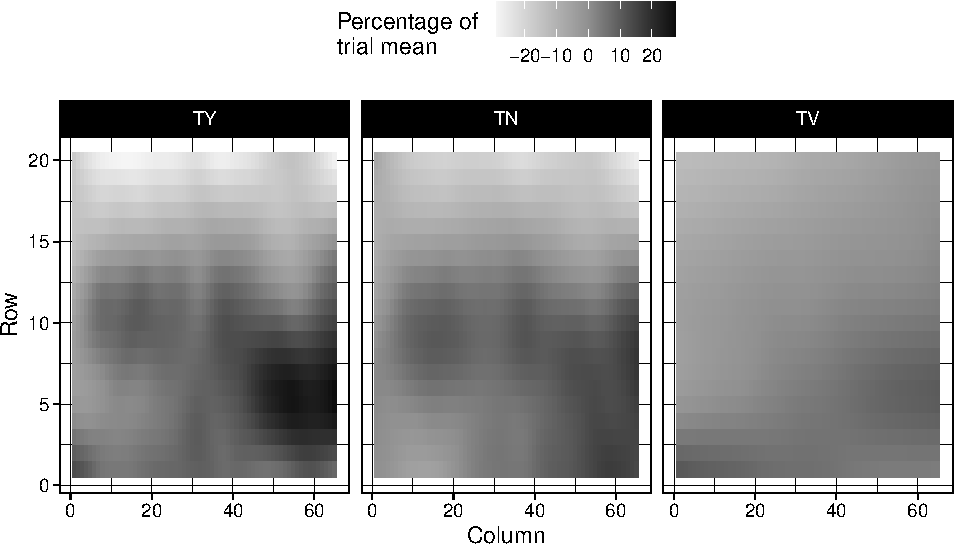
\includegraphics[width=\linewidth]{./figs_02/Fig1.pdf}
\caption{\label{fig:trend-est}Estimated spatial trends scaled by trial mean for total yield (TY; \(\frac{Mg}{Ha}\)) , tuber number (TN; Number of tubers per plot), and tuber volume (TV; Average \(cm^3\) per plot) within the Est screening trial.}
\end{figure}


\section{Results}

\subsection{Spatial Components}\label{spatial-components}

Spatial models for the Est and Heelsum trials were estimated for each yield component. All spatial models successfully converged with credible spatial trends for both trial locations. Model residuals for all environmental models showed little to no evidence of deviation from normality; the following suggest successful delineation of spatial components for all traits in both field trials.

Total yield and tuber number exhibited evidence for strong local trends with a row effect contributing to the spatial trend in Est (Figure \ref{fig:trend-est}). While these same components also impacted tuber volume, it was not nearly so prominent (See S1). The similar magnitude of row effects on tuber number and total yield can also be observed through the ratio of effective and nominal dimensions which were identical for these two traits (0.68) in contrast to tuber volume (0.47). Additionally, the effective nominal dimension ratio for hybrids (i.e.~a generalised heritability) was highest in tuber volume followed by total yield and lastly tuber number (See Table S1).

Overall, the spatial trends in the Heelsum trial were less severe than those evaluated in the screening trial in Est. Interquartile ranges of field effects were between -8.96\% and 9.04\% of the trial mean for total yield in Est while the range was -2.85\% and 3.55\% of the trial mean for yield in Heelsum (Figure \ref{fig:trend-hee}). The differences in magnitude of spatial components between these two trials were also similar for tuber number and tuber volume. Nonetheless, the estimated spatial components did have a modest effect on all yield related components in Heelsum. In particular, random effects for the field column had a minor impact on tuber volume (0.55), tuber number (0.48), and total yield (0.45) (See Table S2). General heritability estimates for Heelsum were akin to those observed in Est with values of 0.9, 0.82, and 0.88 for tuber volume, tuber number, and total yield, respectively.

\begin{figure}
\centering
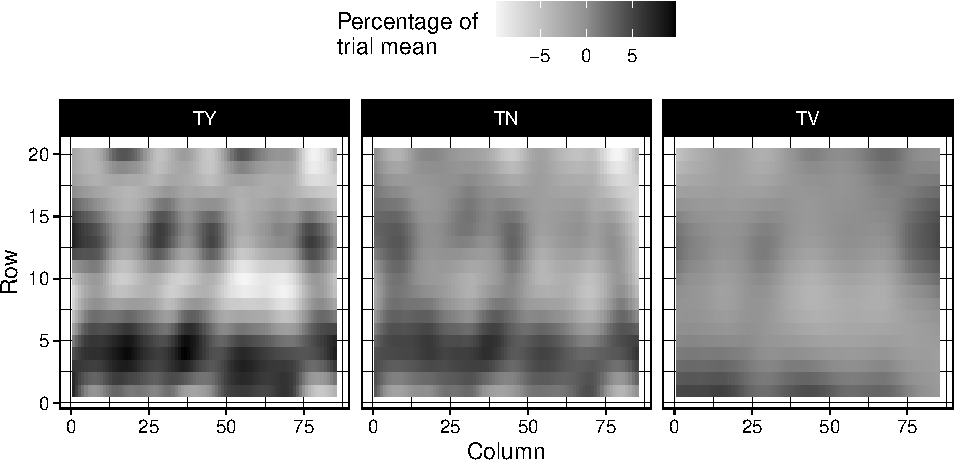
\includegraphics[width=\linewidth]{./figs_02/Fig2.pdf}
\caption{\label{fig:trend-hee}Estimated spatial trends scaled by their trial mean for total yield (TY; \(\frac{Mg}{Ha}\)) , tuber number (TN; Number of tubers per plot), and tuber volume (TV; Average \(cm^3\) per plot) within the Heelsum screening trial.}
\end{figure}

\subsection{Hybrid estimates}\label{hybrid-estimates}

    Using spatially corrected phenotypes from model \eqref{eq:general-spline-model}, we extracted both marginal and conditioned hybrid BLUP's from model \eqref{eq:hybrid} (Figure \ref{fig:blups-plot}). Generally, hybrid performance was far greater in Heelsum over Est. The trial mean for total yield was 13.1 and 22.4 \(Mg \cdot Ha^{-1}\) for Est and Heelsum, respectively. Likewise, average tuber number was 136 tubers in Est and 199 tubers in Heelsum. Trial means for tuber volume were comparatively more stable between trial locations with means of \(21.3~cm^3\) in Est and \(24.2~cm^3\) in Heelsum. Along with differences in mean hybrid performance, there was also greater dispersion of phenotypes in Heelsum than in Est. This was especially apparent for total yield in Heelsum which displayed a standard error twice the size of total yield in Est. This same marked difference could also be seen in tuber number where BLUP's in Heelsum exhibited a standard error 1.6 times greater than that which was found in Est. Tuber volume in contrast to the other phenotypes exhibited similar BLUP distributions between both trial locations. Examining these BLUP's in light of each trait's variance components (See Table S3) suggests that tuber volume showed the greatest stability of all three phenotypes.

    \begin{figure}
    \centering
    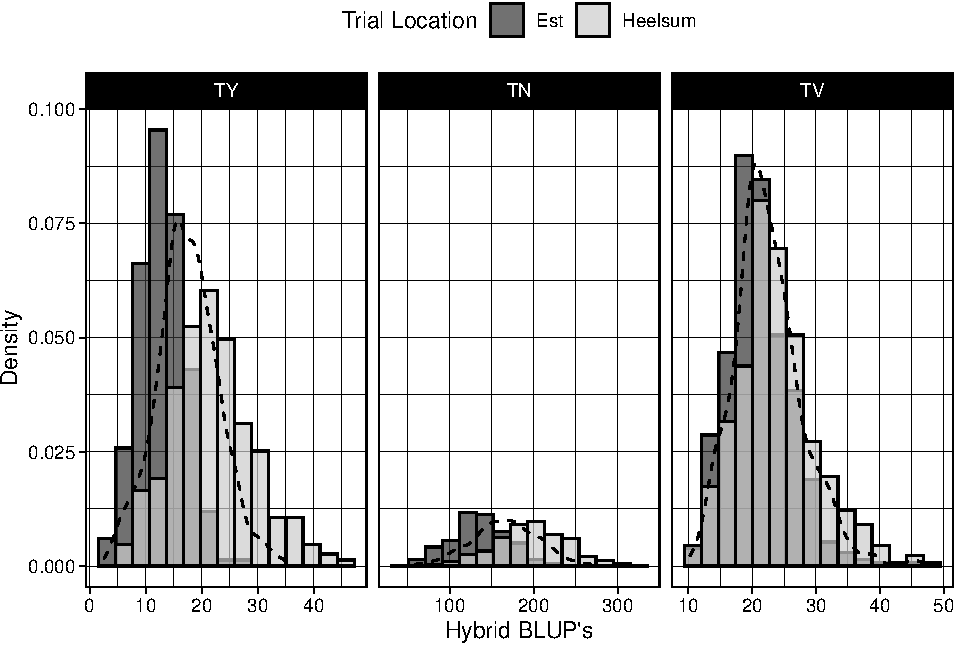
\includegraphics[width=\linewidth]{./figs_02/Fig3.pdf}
    \caption{\label{fig:blups-plot}Hybrid best linear unbiased predictions for total yield (TY; \(\frac{Mg}{Ha}\)) , tuber number (TN; Number of tubers per plot), and tuber volume (TV; Average \(cm^3\) per plot) conditioned on Est and Heelsum trials. Across-location BLUP's visualised through black density curve.}
    \end{figure}

\subsection{Variance Ratios}\label{variance-ratios}

        Variance estimates were derived for all specified random effects for models \(M_0\) and \(M_f\). Tuber volume not only exhibited the largest proportion of variance explained by SCA (\(d^2 = 0.14\)), but also had the largest total genetic variance of any trait (\(H^2 = 0.86\)) (Figure \ref{tab:ratio-tab}). Tuber number and total yield harboured similar proportion's of SCA (\(d^2 = 0.12\)) with a considerable portion of non-additive effects being partitioned in the SCA by environment interaction (Figure \ref{fig:plot-var}). Broad-sense heritabilities were quite similar between tuber number (0.74) and total yield (0.71) with the primary difference between the two traits being the partitioning of genotype by environment interactions (\(\frac{\sigma^2_{ae}}{\sigma^2_{GE}}\) equal to 0.78 in total yield in contrast to 0.65 in tuber number) and size of the residual variance (Figure \ref{fig:plot-var}). The additive genetic component was the largest genetic effect across all traits with the ratio of additive genetic variance being identitical in total yield and tuber number (0.84) and nearly identical in tuber volume (0.83). Between models \(M_0\) and \(M_f\), partitioning of variance changes most drastically for \(\sigma^2_{ae}\). These were much larger in \(M_f\) in tuber number and total yield with the incorporation of the SCA main effect and SCA by environment interaction (Figure \ref{fig:plot-var}).

        \begin{figure}
        \centering
        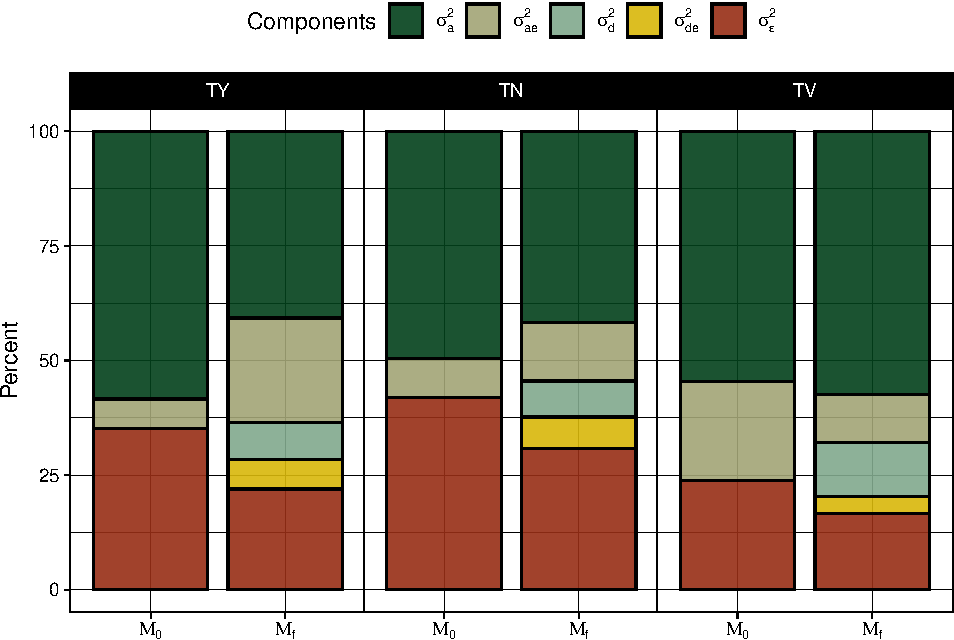
\includegraphics[width=\linewidth]{./figs_02/Fig4.pdf}
        \caption{\label{fig:plot-var}Partitioning of total phenotypic variance into additive (\(\sigma^2_a\)), dominant (\(\sigma^2_d\)), interactive (\(\sigma^2_{ae}\) \& \(\sigma^2_{de}\)), and residual (\(\sigma^2_\varepsilon\)) genetic components across each genetic model (\(M_0\) and \(M_f\)) for total yield (TY), tuber number (TN), and average tuber volume (TV).}
        \end{figure}

        \begin{table}

        \caption{\label{tab:ratio-tab}The broad and narrow-sense heritabilities ($H^2$ and $h^2$, respectively), dominance ratio ($d^2$), proportion of additive genetic variation ($\frac{\sigma^2_a}{\sigma^2_G}$), and proportion of additive genotype by environment interaction over total genotype by environment interaction ($\frac{\sigma^2_{ae}}{\sigma^2_{GE}}$) estimated from the $M_f$ model for total yield (TY), tuber number (TN), and average tuber volume (TV).}
\centering
\begin{tabular}[t]{cccc}
\toprule
 & TY & TN & TV\\
\midrule
$H^2$ & 0.71 & 0.74 & 0.86\\
$h^2$ & 0.59 & 0.62 & 0.71\\
$d^2$ & 0.12 & 0.12 & 0.14\\
$\frac{\sigma^2_{a}}{\sigma^2_G}$ & 0.84 & 0.84 & 0.83\\
$\frac{\sigma^2_{ae}}{\sigma^2_{GE}}$ & 0.78 & 0.65 & 0.74\\
\bottomrule
\end{tabular}
\end{table}

\subsection{Genetic correlations}\label{genetic-correlations}

Along with within-trait variance ratios, genetic correlations were also computed using covariances extracted from model \(M_f\). These were produced for GCA (Figure \ref{fig:gca-coef-full-pairs}) and SCA (Figure \ref{fig:sca-coef-full-pairs}) and are shown together with their BLUP distribution for reference. The GCA intra-class correlation coefficient was found to be highest in tuber volume (0.84) followed by tuber number (0.76) and total yield (0.64) (Figure \ref{fig:gca-coef-full-pairs}). Also noteworthy, large within-trial GCA genetic correlations were found between total yield and each of its yield components, tuber number (0.80) and tuber volume (0.64) according to expectation. Little to no genetic correlation could be found between tuber number and tuber volume (0.06). There were minor discrepancies when comparing each of these with their between-trial genetic correlations counterparts (\(\rho_{TY,TN} = 0.81, \rho_{TY,TV} = 0.65, \rho_{TN,TV}=0.11\)).

\begin{figure}
\centering
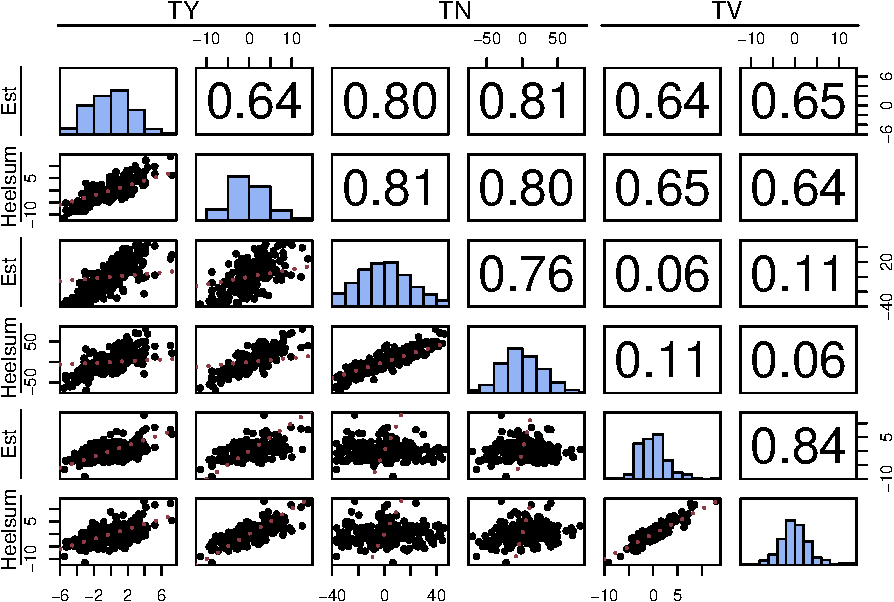
\includegraphics[width=\linewidth]{./figs_02/Fig5.pdf}
\caption{\label{fig:gca-coef-full-pairs}General combining ability pairwise comparisons with scatterplot (lower triangle), genetic correlations derived from \(M_f\)'s variance components (upper triangle), and marginal distributions (the diagonal) of best linear unbiased predictions for total yield (TY; \(\frac{Mg}{Ha}\)), tuber number (TN; total number of tubers per plot), and average tuber volume (TV; \(cm^3\)) in Est and Heelsum. The identity is provided in red for each scatterplot (lower triangle).}
\end{figure}

Similar multivariate trends were observed for SCA genetic correlations, though, with globally smaller values. The SCA intra-class correlation was highest in tuber volume (0.75) with little difference between total yield (0.55) and tuber number (0.53) (Figure \ref{fig:sca-coef-full-pairs}). Relatively large within-trial genetic correlations were observed between total yield and tuber number (\(\rho_{TY,TN} = 0.73\)) and between total yield and tuber volume (\(\rho_{TY,TV} = 0.69\)). Genetic correlations between tuber number and tuber volume were virtually null (\(\rho_{TN,TV}=0.03\)) showing little to no covariance between these two traits for SCA. Examining between-trait between-trial correlations only had minor deviations with respect to within-trial genetic correlations between total yield and tuber number (\(\rho_{TY,TN}=0.76\)) and tuber number and tuber volume (\(\rho_{TN,TV}=-0.01\)); however, these correlations between total yield and tuber volume were distinctly smaller than their within-trial counter-parts (\(\rho_{TY,TV}=0.55\)) (Figure \ref{fig:sca-coef-full-pairs}).

\begin{figure}
\centering
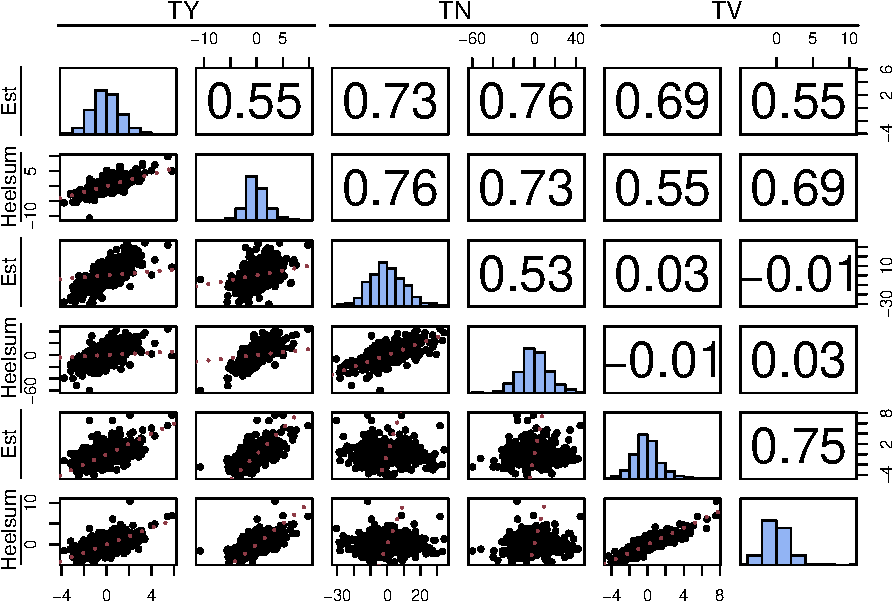
\includegraphics[width=\linewidth]{./figs_02/Fig6.pdf}
\caption{\label{fig:sca-coef-full-pairs}Specific combining ability pairwise comparisons with scatterplot (lower triangle), genetic correlations derived from \(M_f\)'s variance components (upper triangle), and marginal distributions (the diagonal) of best linear unbiased predictions for total yield (TY; \(\frac{Mg}{Ha}\)), tuber number (TN; total number of tubers per plot), and average tuber volume (TV; \(cm^3\)) specific combining ability in Est and Heelsum. The identity is provided in red for each scatterplot (lower triangle).}
\end{figure}

When comparing the GCA and SCA quantiles for each trait and trial location, the GCA BLUP's were consistently larger than those SCA BLUP's. On average, any given GCA quantile was two times larger than its respective SCA quantile; this was true for all traits measured here (See Table S4). These differences in magnitude between the estimated GCA and SCA effects could also be readily seen while examining the size of each variance component (Figure \ref{fig:plot-var}) or even through a simple regression of hybrid BLUP's on the mid-parent value (Figure \ref{fig:bv-sca}). No linear relationship could be found between the estimated GCA and SCA effects for any trait (See Figure S1) coinciding with our model assumptions in   \eqref{eq:sca-model}.

\begin{figure}
\centering
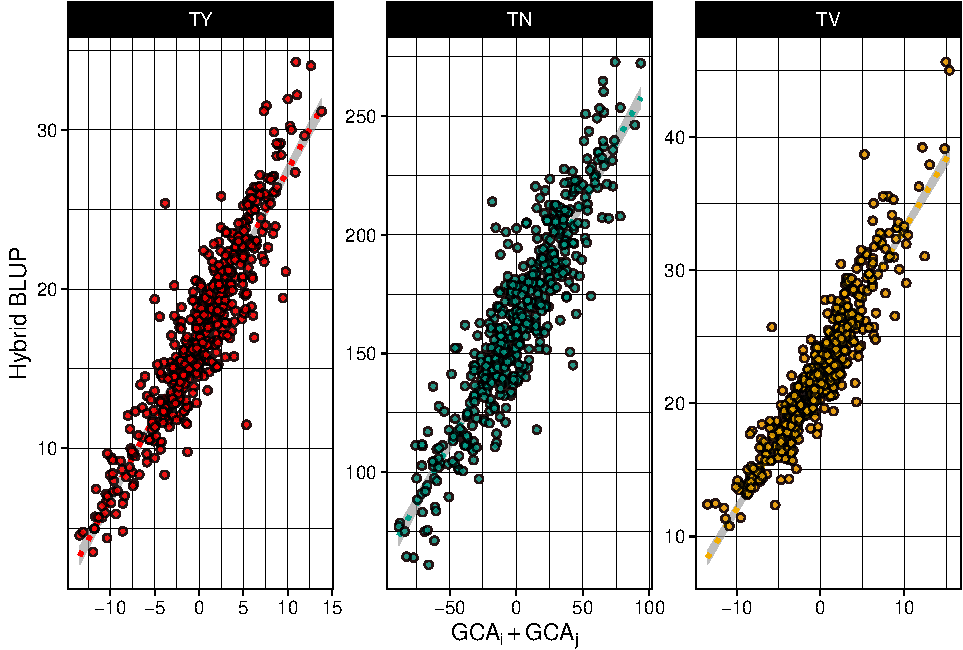
\includegraphics[width=\linewidth]{./figs_02/Fig7.pdf}
\caption{Scatterplot of hybrid BLUP's regressed on the GCA's of parents' i and j for total yield (TY; \(\frac{Mg}{Ha}\)), tuber number (TN; total number of tubers per plot), and average tuber volume (TV; \(cm^3\))}
\label{fig:bv-sca}
\end{figure}

\subsection{Model Testing}\label{model-testing}

The likelihood ratio tests conducted between model \(M_f\) and \(M_0\) was found to be significant yielding a probability less than 0.001 (Table \ref{tab:model-comparison}). This test was also conducted on the univariate equivalent of these models for each trait (\(M_{df}\) and \(M_{d0}\)) and were all found to be significant as well. Each test conformed with the AIC's of each model pair where the smallest AIC was observed in the full genetic model suggesting that the best fit was achieved with the inclusion of SCA and its environmental interaction. This at the very least lend a statistical justification for these non-additive genetic effects in all three tuber traits.

\begin{table}

\caption{\label{tab:model-comparison}Likelihood ratio tests for $M_0$ and $M_f$ genetic models together with each model's Akaike's information criterion for the Multi-trait model (MT), total yield (TY), tuber number (TN), and average tuber volume (TV).}
\centering
\begin{threeparttable}
\begin{tabular}[t]{cccc}
\toprule
 & AIC & $\Lambda(y)$ & $\mathrm{P}(\Lambda(y))$\textsuperscript{\dag}\\
\midrule
\addlinespace[0.3em]
\hline
\multicolumn{4}{l}{\textbf{MT}}\\
\hspace{1em}$M_0$ & 26665 & 586 & ***\\
\hspace{1em}$M_f$ & 26103 &  & \\
\addlinespace[0.3em]
\hline
\multicolumn{4}{l}{\textbf{TY}}\\
\hspace{1em}$M_0$ & 7992 & 132 & ***\\
\hspace{1em}$M_f$ & 7864 &  & \\
\addlinespace[0.3em]
\hline
\multicolumn{4}{l}{\textbf{TN}}\\
\hspace{1em}$M_0$ & 15778 & 92 & ***\\
\hspace{1em}$M_f$ & 15690 &  & \\
\addlinespace[0.3em]
\hline
\multicolumn{4}{l}{\textbf{TV}}\\
\hspace{1em}$M_0$ & 7008 & 235 & ***\\
\hspace{1em}$M_f$ & 6778 &  & \\
\bottomrule
\end{tabular}
\begin{tablenotes}
\item[\dag] ***: $\mathrm{P}(\Lambda(y))< 0.001$
\end{tablenotes}
\end{threeparttable}
\end{table}

\section{Discussion}\label{discussion}

\subsection{Presence of additive vs.~non-additive effects}\label{presence-of-additive-vs.-non-additive-effects}

SCA was detected across all phenotypes (Table \ref{tab:model-comparison}) warranting sufficient evidence that SCA can impact yield, especially in its simpler components, seen primarily in tuber volume (Figure \ref{fig:plot-var}). However, the magnitude of GCA effects were far greater than the magnitude of SCA's estimated across all traits irrespective of the their heritability or size of SCA variance. The GCA quantiles were between 1.4 to 2.5 times larger than their respective SCA quantiles (See Table S4) suggesting a systematic importance of the additive genetic effects in this DHP population. The implications then is that most of the variation in the progeny can be found through the additive genetic variation in the parents. This was most apparent for tuber volume (\(h^2 = 0.71\)) where regression of hybrid performance on the combination of parental GCA's had the best fit of all traits (Figure \ref{fig:bv-sca}). This illustrates that the parental GCA's (or, identically, the mid-parent value) capture the majority of a hybrid's phenotype.

While this study is the largest of its kind, it is certainly not alone in attempting to decompose genetic components of yield in potato. A number of similar populations were used in both diploid and tetraploid backgrounds with wide-ranging results. Many of these studies came to find little non-additive genetic variation for yield components similar to the results presented here with GCA being the primary component for traits like average tuber weight, tuber shape, total tuber number, and total yield \citep{Veilleux1981, Brown1989, Neele1991}. These studies utilised either variants of a diallel or factorial crossing schema making the structure of their statistical models not altogether different than the modelling endeavoured here. One exception between models' \eqref{eq:gca-model} and \eqref{eq:sca-model} and those used in the aforementioned tetraploid populations is that variance attributed to GCA has a different interpretation due to differences in ploidy and levels of inbreeding. This said, there is a large body of work which also finds SCA to be the largest (and at times, the only) detected effect in several complex traits. The same previously mentioned traits as well as others like incidence of hollow heart and tuber uniformity were also found to be predominately under the control of SCA \citep{Killick1977, Veilleux1981, Thompson1984, Haynes2001}. Most notably, \citep{Tai1976} was only able to detect SCA in their partial diallel crosses with no GCA component found for marketable yield and marketable tuber number.

The lack of an empirical consensus on the predominance of GCA and SCA in potato is not very surprising in of itself. The estimation of these parameters are very much contingent on numerous factors including crop ploidy, genetic background, number of parents, degree of environmental stress, and choice of statistical model (to name a few), all of which are prone to change across experiments. Even making comparisons between studies utilising very similar genetic backgrounds can lead to divergent findings \citep{Tarn1977, Maris1989}. While seemingly incoherent, the following does offer some interesting grounds for considering those genetic effects observed here. Many of the aforementioned studies estimated variance components on populations which had undergone siginificant selection through a recurrent selection schema \citep{Haynes2001, Maris1989} or were themselves the product of strong selection on GCA's in their ancestors \citep{Tai1976}. In both cases, less additive genetic variation can be expected among hybrids derived from them leaving non-additive genetic variation to be the predominant genetic effect within their inter-population crosses. Conversely, populations like ours which show ample additive genetic variation might be younger with respect to selection pressure in their ancestors on these traits; though without any formal analysis on population structure this is speculative. Another line of reasoning for the smaller SCA's found here relative to many of the tetraploid studies could be explained by \emph{progressive heterosis} whereby higher order non-additive genetic effects become possible through polyploidy \citep{Birchler2003}. Recent genomic studies in tetraploid potato support this hypothesis with evidence of a genetic residual effect (which could be explained by tri \& quadrigenic dominance) contributing as much as 45\% of total genetic variation in potato yield \citep{Endelman2018}. However, making any meaningful confirmation on the specific role of ploidy in producing non-additive genetic effects is beyond the scope of this present study and only deserves a cursory mention.

\subsection{Genetic Architecture of yield}\label{genetic-architecture-of-yield}

Among our two yield components (i.e. tuber number and and average tuber volume), we found strong genetic correlations between each and total yield for both the additive (see Figure \ref{fig:gca-coef-full-pairs}) and non-additive genetic effects (see Figure \ref{fig:sca-coef-full-pairs}). Numerous studies have identified these same phenotypes as major determinants of total tuber yield marking them both as strategic heritable targets for breeding \citep{Khayatnezhad2011, Thompson1984}. Consistent with these studies, tuber number GCA's appeared to impact total yield more than tuber volume with \(\rho_{TN,TY}\) equalling 0.80 and a \(\rho_{TV,TY}\) of 0.64. SCA genetic correlations behaved similarly with \(\rho_{TN,TY}\) equal to 0.73 and \(\rho_{TV,TY}\) equal to 0.69. Interestingly, while tuber volume had the greatest stability with respect to both GCA (\(ICC_{gca}=0.84\)) and SCA (\(ICC_{sca}=0.75\)), the between-trial genetic correlations in \(\rho_{TV,TY}\) dropped to 0.55 suggesting less coupling in SCA by trial response with total yield in contrast to the between-trial genetic correlations seen in total yield and tuber number (\(\rho_{TN,TY}\)=0.76). These additive and non-additive components point to tuber number being the primary determinant of yield in this hybrid population.

Among certain market classes, our two yield components, average tuber volume (or tuber size) and tuber number, often exhibit an inverted relationship due to the physiological and genetic limits of potato. For example, \citep{Thompson1984} found a genetic correlation of -0.24 among their panel. Additionally, \citep{Lemaga1990} identified negative cubic trends between tuber number and average tuber weight capturing a majority of variation. Interestingly, no meaningful relationship could be found between these two yield components with respect to additive (Figure \ref{fig:gca-coef-full-pairs}) and non-additive genetic correlations (Figure \ref{fig:sca-coef-full-pairs}). To repeat our previous suspicion, this suggests a lack of directional selection on one of these two traits evident by the lack of genetic constraints between them \citep{Blows2009}. Tuber volume had the largest proportion of additive variation (Figure \ref{fig:plot-var}) and genetic variation in general (Table \ref{tab:ratio-tab}) suggesting little to no direct selection on this component of yield. These properties then make this population an interesting candidate for future selection given its genetic potential to be adapted to a variety of tuber types. Another oddity to consider here is that while SCA was detected independently in these two yield components, this did not manifest in the increase of SCA in total yield, but very much the opposite. Others have identified that heterosis in these same yield components were responsible for a geometric increase in gross yield \citep{Tarn1977}. Further multivariate studies of vigour in diploid potato could further elucidate SCA architecture especially as selection pressure is applied, a key scenario within breeding programmes.

\subsection{Using GCA \& SCA in commercial breeding}\label{using-gca-sca-in-commercial-breeding}

The large narrow-sense heritabilities and magnitude of the GCA's found here have major implications for breeders of DHP. To begin, the valid estimation of GCA's further validate the potential of potato in its conversion into a inbred-hybrid crop as purported before \citep{Jansky2016, Lindhout2011}. Further, the size of the estimated GCA's relative to a hybrid's average performance (Figure \ref{fig:bv-sca}) show that standard breeding designs used in other hybrid crops will likely be just as efficacious in DHP. For example, the use of test crosses, a mainstay in maize breeding, can also be utilised in evaluating performance of potato parental lines for hybrid crosses with reasonable success. These test crosses can be further utilised for model training and be the basis for genomic selection of parents (using breeding values) or hybrid crosses (via mid-parent value); again, a standard-place method in hybrid breeding \citep{Albrecht2011}. To quickly add, while we found little contributions made by SCA, their relevance to breeders do not necessarily end here. Depending on the specific mechanism behind these observed non-additive effects, they could be further exploited in the trait of interest through initial breeding design (e.g.~formation of heterotic pools). Heterotic breeding has become a major target for quality trait improvement in other solanaceous crops including chilli pepper \citep{Herath2020}, eggplant \citep{Kumar2020}, and tomato \citep{Pearson1983}. This is where potato meets an interesting intersection between the vegetable and agronomic worlds where SCA might play a more valuable role for qualities controlling specific market criteria (e.g.~average tuber volume, tuber length \& shape) but would be less emphasised in composite and complex traits (e.g.~gross yield, starch \& protein content) where GCA is the predominant genetic effect at play. Having said this, future work into the biometric mechanism of vigour will be able to lend more wisdom for how breeders should wield this in a hybrid potato breeding programme.



\section{Conclusion}\label{conclusion}

\subsection{Limitations}\label{limitations}

The application of these results should be done with some qualification. One principal limitation of this study can be found in the number of trials conducted. All inference drawn here was based upon only two trials which took place over one season. This limits our findings to one particular year which narrows their interpretive weight and scope. Related to this, this study was performed on a particular composite experimental population and does not necessarily represent the heterotic potential of the tuber-bearing Solanum genepool. Considering all this, this population is an appropriate candidate for the purpose of surveying the presence and potential of heterotic vigour in DHP which was the aim of this current paper. 

\subsection{Future work}\label{future-work}

Finding evidence for heterotic effects in DHP does not yield much regarding the source of the effects identified here. The statistical models assume all underlying effects captured by the SCA term to be the product of cumulative dominance deviations across the genome, but there exists many other plausible sources of non-additive variation. Since its conception, genetic theory has explained heterosis with a whole suite of models with many being broadly plausible (See \citep{Labroo2021}). However, these apparent non-additive effects could just as simply be explained by dispersion of additive alleles among parents, a hypothesis which is generally supported empirically \citep{Pearson1983, Mackay2021}. Nevertheless, these effects continue to be interesting point of study and still remain an important target in hybrid breeding of modern crops. This is especially worthwhile in DHP given its novelty as a hybrid crop with the potential of heterotic breeding to still be determined.


This is the first study in diploid hybrid potato to produce estimates of general and specific combining abilities using a large panel of commercially-derived parents. This represents a major milestone in the reorientation of potato from a clonal tetraploid to a diploid inbred-hybrid crop. Identifying the predominance of additive genetic effects for multiple yield components among hybrids offers strategic insight on the necessity of effective generation of parental lines and early population development in general. Though the estimated non-additive effects in this population are smaller in contrast to their additive counterparts, heterotic vigour shows some minor role in simpler traits. Specific quantitative traits should be targeted for SCA exploitation to bolster variety development on top of their parental effects. Further research into the genetic mechanisms for the apparent non-additive effects will also better elucidate the strategic advantage (if any exist) in key economic targets in hybrid potato.

\section{Data availability}

All trial and pedigree data utilised for the following analysis have been made
available on GSA FigShare. File Phenotypes.csv contains the three afore-
mentioned traits along with field trial row, column, and block indices for each
observation. File Pedigrees.csv gives a hybrid identification number with
each parental code.

\section{Acknowledgments}
Acknowledgments should be included here.

\section{Funding}
Funding, including Funder Names and Grant numbers should be included here.

\section{Conflicts of interest}

The authors of this publication have no conflicts of interest to report related to the the results of this study or the inferences, speculation,\& conclusions derived from them.


\include{03_refsrefschapter3}
\include{04_chapter4}
\include{05_chapter5}
\chapter[Synthesis]{Synthesis}
\chaptermark{Synthesis}
\label{cha:Chapter6}
\newpage

“A machine does not care”
― Tom Godwin, The Cold Equations

Lorem ipsum dolor sit amet, consectetur adipisicing elit, sed do eiusmod
tempor incididunt ut labore et dolore magna aliqua. Ut enim ad minim veniam,
quis nostrud exercitation ullamco laboris nisi ut aliquip ex ea commodo
consequat. Duis aute irure dolor in reprehenderit in voluptate velit esse
cillum dolore eu fugiat nulla pariatur. Excepteur sint occaecat cupidatat non
proident, sunt in culpa qui officia deserunt mollit anim id est laborum.
 % Discussion


\backmatter
\bibliographystyle{model5-names}
\phantomsection
\addcontentsline{toc}{chapter}{References}
\bibliography{library}
\fancyhead{}

\cleardoublepage
\phantomsection

%% Back Matter
\phantomsection
\chapter{About the author}

Lorem ipsum dolor sit amet, consectetur adipisicing elit, sed do eiusmod
tempor incididunt ut labore et dolore magna aliqua. Ut enim ad minim veniam,
quis nostrud exercitation ullamco laboris nisi ut aliquip ex ea commodo
consequat. Duis aute irure dolor in reprehenderit in voluptate velit esse
cillum dolore eu fugiat nulla pariatur. Excepteur sint occaecat cupidatat non
proident, sunt in culpa qui officia deserunt mollit anim id est laborum. Lorem ipsum dolor sit amet, consectetur adipisicing elit, sed do eiusmod
tempor incididunt ut labore et dolore magna aliqua. Ut enim ad minim veniam,
quis nostrud exercitation ullamco laboris nisi ut aliquip ex ea commodo
consequat. Duis aute irure dolor in reprehenderit in voluptate velit esse
cillum dolore eu fugiat nulla pariatur. Excepteur sint occaecat cupidatat non
proident, sunt in culpa qui officia deserunt mollit anim id est laborum.


\section*{Peer-reviewed journal publications}

% Full citation of publication 1
% This refers to the article key in the refs.bib file.
\bibentry{Adams2022}

Full citation of publication 2


\section*{Peer-reviewed book chapter}

Book chapter 1

Book chapter 2

\section*{Other scientific publications}

Conference publication 1

Conference publication 2

\cleardoublepage
\phantomsection

\include{08_TESF}

\renewcommand{\headrulewidth}{0pt}
\cleartoleftpage

\include{09_funding}
\end{document}
